\chapter{Introduction}

Autonomous robots are robotic devices capable of performing tasks based on inputs from various types of sensors, without human interaction. Much research in the recent years has focused on the development of autonomous cars (also known as Unmanned Automobiles) which can drive without interaction from the driver, but just by sensing the environment. This is an interesting field, as it may lower the number of traffic accidents and especially reduce the traffic congestion in bigger cities by providing a better traffic flow.

In this present project we designed and constructed an autonomous robot, capable of following a line by using a mixture of cameras and IR sensors for gathering input about the surroundings. Close attention was paid to the use of camera sensing and image processing for detecting and extracting the line. The traditional method has been to use an array of photo-sensors, but due to the low resolution, an alternative method is necessary for archiving a better stability.

This paper outlines the work done, and shows how a camera can be used instead of a traditional array of photo sensors. Further more, as an additional feature, it is explained how the live image data is streamed to a computer, for a live preview of what the `robot sees`.

Our robot may in the following chapters be referred to as `the robot`, `the system` or simply `Eyebot`.
TODO More attention to traffic accidents, traffic flow and congestion.

%
%
%
%
\section{Subsystems and Block Diagram}

The robot consist of several subsystems, which have different responsibilities. The block diagram in figure \ref{fig:intro_1}, outlines the basic components of the system with connections betweens them. 

\begin{figure}[!h]
	\centering
	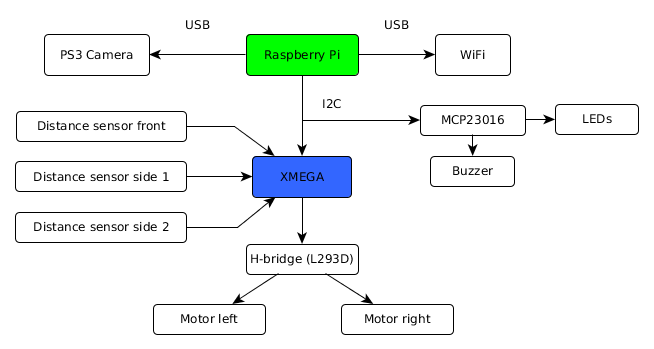
\includegraphics[width=1\textwidth]{resources/Blockdiagram}
	\caption{Block diagram of the subsystems}
	\label{fig:intro_1}
\end{figure}

As seen on the block diagram, the main processor of the system is an ARM-based Raspberry Pi computer. The Raspberry Pi first of all acts as the overall state machine when driving the track. It knows when to follow the line, go to the wall, rotate and so on (more on that in chapter \ref{chap:track}). Moreover the Raspberry Pi takes care of capturing images from the camera, processing the images, and calculating the error signals when following the line. As an additional feature, the live image data when following the line, are transmitted over WiFi to a laptop, for live preview of the robot's processed and annotated image. The image capture and processing is discussed in detail in chapter \ref{chap:camera}. 

Below the Raspberry Pi, an Atmel XMEGA192C micro-controller is responsible for powering and controlling the motors. The XMEGA is instructed directly by the Raspberry Pi, by commands received over the I2C (Two Wire Interface) bus. Equally important the XMEGA reads analog signals from the three distance sensors, and makes them available for the Raspberry Pi through the I2C bus. The motor-controller is discussed in chapter \ref{chap:motors} and the distance sensors are discussed in chapter \ref{chap:wall_dist}.

As an additional feature, the robot has an array of LEDs mounted on its bumper, and a buzzer for indicating state changes. Those are powered by an MCP23016 I/O expander chip, that communicates with the Raspberry Pi using I2C. This subject will not receive any more attention in the report than this.

%
%
%
%
\section{Requirements Specification}
\subsection{Assumptions}

We assume an average speed for the robot of 1 m/s. By looking at the line, we found that it should be
reasonable to make corrections every 0.1 m. This gives an maximum cycle time of 100 ms. Cycle
time includes capturing and processing of the image, calculation of the error and correction value,
transmitting the corrective actions to the motors, and waiting for the motors to respond and react.
By tilting the camera forward, we might be able to detect future obstacles, and take required actions
such as slowing down.

\subsection{Formal requirements}
\begin{enumerate}
\item The robot should be able to follow the track on first floor. This includes 
\begin{itemize}
\item Make a decision on which way to turn when seeing the line first time
\item When a short peace of tape intersects the line, the robot should turn 90 degrees to the left
and drive towards the wall. It should stop 20 centimeters from the wall, turn 180 degrees
(TBC) and go back and follow the line as usual.
\item When a short line is sensed on the left side of the line, the robot should speed up, and try to go as fast as possible for the rest of the track.
\item At the end of the track, the robot should drive to the wall, keeping a distance of 20
centimeters to the wall, and then follow the wall to the end of the track.
\end{itemize}
\item The robot should be able to drive at a maximum speed of 1 m/s (TBC).
\item The robot should make corrections every 0.1 m (TBC), which is every 100 ms (TBC) at 1 m/s.
\item The line should be sensed using a camera and image processing (TBC).
\item A Raspberry PI should be the main controller in the system.
\item The Raspberry PI should capture images of the floor, analyse the image, and calculate the error.
\item The motors should be controlled by an AVR microcontroller, that interfaces the Raspberry PI
using I2C (TWI).
\item The speed of the motors should be controlled using PWM signals through a H-bridge.
\item The distance to the wall should be measured using a distance sensor in the front, and one or more on the
left side of the robot.
\end{enumerate}



\section{Time Schedule}

